%-----------------------------------------------------------------------------
%
%               Template for sigplanconf LaTeX Class
%
% Name:         sigplanconf-template.tex
%
% Purpose:      A template for sigplanconf.cls, which is a LaTeX 2e class
%               file for SIGPLAN conference proceedings.
%
% Guide:        Refer to "Author's Guide to the ACM SIGPLAN Class,"
%               sigplanconf-guide.pdf
%
% Author:       Paul C. Anagnostopoulos
%               Windfall Software
%               978 371-2316
%               paul@windfall.com
%
% Created:      15 February 2005
%
%-----------------------------------------------------------------------------


\documentclass[preprint,numbers,numberedpars,10pt]{sigplanconf}

% The following \documentclass options may be useful:

% preprint      Remove this option only once the paper is in final form.
% 10pt          To set in 10-point type instead of 9-point.
% 11pt          To set in 11-point type instead of 9-point.
% numbers       To obtain numeric citation style instead of author/year.

\usepackage{amsmath}

\newcommand{\cL}{{\cal L}}

\usepackage{listings}
\usepackage{color}
\usepackage{textcomp}
\usepackage{graphicx}
\usepackage{stmaryrd}
\usepackage{caption}
\usepackage{mathtools}
\usepackage[lite,subscriptcorrection,slantedGreek,nofontinfo]{mtpro2}

\lstset{language=Scheme}
\definecolor{codegreen}{rgb}{0,0.6,0}
\definecolor{codegray}{rgb}{0.5,0.5,0.5}
\definecolor{backcolour}{rgb}{0.95,0.95,0.92}
 
%\bibliographystyle{abbrvnat}
%\setcitestyle{sorting=none}  %super,open={[},close={]}}

\begin{document}

\special{papersize=8.5in,11in}
\setlength{\pdfpageheight}{\paperheight}
\setlength{\pdfpagewidth}{\paperwidth}

\conferenceinfo{CONF 'yy}{Month d--d, 20yy, City, ST, Country}
\copyrightyear{20yy}
\copyrightdata{978-1-nnnn-nnnn-n/yy/mm}
\copyrightdoi{nnnnnnn.nnnnnnn}

% Uncomment the publication rights you want to use.
%\publicationrights{transferred}
%\publicationrights{licensed}     % this is the default
%\publicationrights{author-pays}

\titlebanner{This paper is a draft}        % These are ignored unless
\preprintfooter{short description of paper}   % 'preprint' option specified.

\title{Multi-purpose web framework design based on websocket over HTTP Gateway}
\subtitle{A case study on GNU Artanis}

\authorinfo{Mu Lei}
           {SZDIY Community}
           {mulei@gnu.org}

\maketitle

\begin{abstract}
  The traditional Internet communication is largely based on HTTP protocol, which provides hyperlinked, stateless exchange of information.
  Although HTTP is convenient and easy to understand, it's problematic for real-time data exchange. The websocket protocol is one of the way
  to solve the problem. It reduces overhead and provides efficient, stateful communication between client and server \citep{6197172}.
  
  This paper introduces a web framework design in Scheme programming language, which takes advantage of websocket protocol to provide both
  convenience and efficiency. In spite of the expressiveness, Scheme provides powerful abstract ability to implement coroutines with
  continuations for the server core.
  It is proved that continuations could be the model for directly expressing concurrency in Scheme language \citep{shivers1997continuations}.
  In this paper, we'll take GNU Artanis as a study case to indicate the same purpose. Moreover,
  GNU Artanis uses GNU Guile which is a practical Scheme implementation which provides delimited continuations for better implementing coroutines.

  GNU Artanis also provides useful modules for web programming, RESTful, web caching, templating, MVC, and a novel abstraction for relational
  mapping to operate databases. We'll give it a summary in the rest of the paper.
\end{abstract}

\category{D.3.3}{Programming Languages}{Language Constructs and Features}[Frameworks]

% general terms are not compulsory anymore,
% you may leave them out
\terms
Scheme, framework

\keywords
Scheme, web framework, websocket, delimited continuation, coroutine

\section{Introduction}

Web framework is a library for rapid prototyping web development, and usually provide CLI (Command Line Interface) or
GUI (Graphical User Interface) tools to generate code for reducing workload according to certain patterns specified by the developers.
In spite of using web specific language such as PHP, the older approach for web programming is CGI (Common Gateway Interface).
Although many people think CGI is outdated, it is simple to understand and easy to use.
It can yet be regarded as a practical way for web programming.

But the industry always requires more: a fast way for rapid prototyping, an approach for both productivity and reliability, clean and DRY
(Don't Repeat Yourself) for maintaining, high level abstract for hiding details, less coding, securities, etc.
Most of the modern web frameworks such as Ruby on Rails provides the tools necessary to produce a web application model,
which is the underlying program itself \citep{1597080}. 

This paper will use the term {\it HTTP Gateway} to indicate the unified connection management interfaces and verification methods of websocket
over HTTP. The {\it HTTP Gateway} is not a new concept, actually it's hidden in many server design. It is worth to discuss it explicitly,
for it is important to understand how GNU Artanis manages all the websocket connections. We'll mention it in \ref{HTTP Gateway}.

Besides, this paper will show a different way to implement concurrent server. It is different from the callback way used in C or Node.js.
We use continuations which has been already practiced as the abstract of concurrent processes in several cases
\citep{Krishnamurthi2007}\citep{Hieb:1990:CC:99164.99178}\citep{Hieb:1994:SUB:184324.184330}.
In this paper, we'll show a new way with the feature named delimited continuations, which is better abstract than traditional continuations.
We'll discuss it in \ref{Delimited Continuations}.

The C10K and C10M problem told us that the performance is not the only thing to concern for high concurrent server, but also the scalability.  
The old method to use select() or poll() has $O(n)$ complexity, which is the handicap to hold more connections \citep{lemon2001kqueue}.
The new method is kqueue()/epoll()/IOCP which has O(1) complexity to query available connection sockets. We'll take epoll() as an example to
discuss the scalability issue in \ref{Non-blocking with Epoll}.

The websocket is a protocol for two-way communication between client and server over TCP connection. The client is, in a broad sense,
unnecessary to be a web browser. One of the benefit of websocket is that the developers could take advantage of TLS used in HTTPS for
encryption. And another is that unified listening port for arbitrary services. We will discuss websocket in \ref{Websocket}.

Finally, we'll discuss some of the notable features of GNU Artanis in \ref{Some features in GNU Artanis}.
%. 

%\includegraphics{mmr.eps}
%\lstinputlisting{tt.scm}

\section{Some background knowledge}
\subsection{Continuations}

\begin{figure}[tbph]
  %\centering
  \raggedright
  \label{fig:cont_sema}
  \begin{align*}
    \shortintertext{ {\it variable}: }
    \llbracket{x}\rrbracket\rho \quad&=\quad \lambda{\kappa}.(\kappa \: (\rho \: x))
    \\\
    \shortintertext{ {\it $\lambda$\textendash abstract}: }
    \llbracket{\lambda{x}.M}\rrbracket\rho \quad&=\quad
    \lambda{\kappa}.\kappa\:(\lambda{v}.\lambda{\kappa'}.\llbracket{M}\rrbracket\:(\rho[x \mapsto v])\:\kappa'))
    \\\
    \shortintertext{ {\it application}: }
    \llbracket{M N}\rrbracket\rho \quad&=\quad
    \lambda{\kappa}.\llbracket{M}\rrbracket\rho\:(\lambda{m}.\llbracket{N}\rrbracket\rho\:(\lambda{n}.((m\:n)\:\kappa)))
  \end{align*}
  \caption{Continuation Semantics in spirit of Fischer’s CPS transform.}
\end{figure}

The $\llbracket{...}\rrbracket$ means a simplified one-pass CPS transformation, which should be constrained by two conditions:
$(1)$ Shouldn't introduce any administrative redex (the reducible expression operated by a continuation capturing lambda);
$(2)$ Wouldn't reduce the source term. And $E[...\mapsto...]$ means capture-avoiding substitution in expression $E$.


\subsubsection{Delimited Continuations} \label{Delimited Continuations}

Delimited continuations are more expressive than traditional abortive continuations.

As an ordinary continuation stands for ``the rest of the computation'', a delimited continuation represents
``the rest of the computation up to somewhere'' \citep{sumii2000implementation}.

(Write something principle about delimited continuations)

(The reason why use delimited continuations)
Delimited continuations has been implemented in few languages: GNU Guile, PLT Scheme, Scheme48, OCaml, Scala.
Considering that many mainstream dynamic languages has first class continuations (call/cc), optimistically, it is possible that more languages
will implement delimited continuations too. In view of above mentioned reasons, the study case in this paper may shed some light on server
design problem in the future.

\subsection{Coroutines}

Coroutines are essentially procedures which saves states between calls. It has become very important form of concurrency, and avoid practical
difficulties (race conditions, deadlock, etc) to reduce complexities. Developers are unnecessary to take care of synchronization by
themselves, but leave it to this paradigm as its built-in feature. Coroutines is not generic enough to solve any concurrency problem, however,
it's idea solution for server-side development.

It is demonstrated that coroutines may easily be defined by users given first class continuations\citep{Haynes:1984:CC:800055.802046}. The
term ``first class'' here means a continuation could be passed and returned from functions, and stored in a data structure with indefinite
extent. The coroutine could be implemented as a procedure with local state. In server-side development, in spite of traditional HTTP requesting,
most servers need to maintain long live session for a connection. It is required that these procedures could be broken for a while, and sleep
to the time when next packet arrives. In old fashion, people uses OS level threads (say, pthread) to avoid blocking. But it brings some
critical overheads (trap into kernel, locks, synchronization), no mention the difficulties in debugging programs with threads. Ironically,
it is even complained by people that threads model is bad idea for practices\citep{ousterhout1996threads}.

Since Scheme provides full support for continuations, implementing coroutines is nearly trivial, requiring only that a queue of continuations
be maintained. Moreover, this paper introduce the way to implement coroutines with delimited continuations. We'll see how this approach is
convenient and clean later in this section.

As described in \ref{Delimited Continuations}, GNU Guile provides several similar abstract interfaces to handle delimited continuations.
Here we choose the pair functions {\it call-with-prompt} and {\it abort-to-prompt} for it, since it's easier to invoke scheduler procedure
which is used to resume the stopped coroutines while throwing the delimited continuations.

The basic principle of coroutine implementation is that saving context to a first class object then adding it into a queue, and scheduling
around till the queue is empty. So the first step is to initialize a queue:

\begin{lstlisting}
(define *work-queue* (new-queue))
\end{lstlisting}

And the {\it spawn} interface, it's common to spawn a new coroutine. The {\it call-with-prompt} function was introduced in
\ref{Delimited Continuations}.

\begin{lstlisting}
(define-syntax-rule (spawn body ...)
 (call-with-prompt
  (default-prompt-tag)
  (lambda ()
   body ...)
  save-context))
\end{lstlisting}

As described in \ref{Delimited Continuations}, the last argument of {\it call-with-prompt} is a function which receives current continuation
as the first argument. Obviously, we should save it to the queue for it needs to sleep. The second argument is optional, and we customize it
as the index of the request in our example.

\begin{lstlisting}
(define (save-context k idx)
 (format #t
         "Request~a EWOULDBLOCK!~%"
         idx)
 (queue-in! *work-queue* (cons idx k)))
\end{lstlisting}

The sleeping feature is implemented with {\it abort-to-prompt}. When it's called, the runtime will throw the current continuation bound to
{\it k} as the first argument of {\it save-context} function.

\begin{lstlisting}
(define-syntax-rule (coroutine-sleep idx)
 (abort-to-prompt
  (default-prompt-tag)
  idx))
\end{lstlisting}

Each time when certain condition were met, the related delimited continuation would be resumed. The {\it resume} function will resume the task
properly. Note that the resumed continuation should be re-delimit again to avoid stack issues. And when calling {\it k} for resuming continuations,
it is necessary to pass {\it idx} as the argument.

\begin{lstlisting}
(define-syntax-rule (resume k idx)
 (call-with-prompt
  (default-prompt-tag)
  (lambda ()
    (k idx))
  save-context))
\end{lstlisting}

Finally, we need a scheduler to arrange all the tasks to be completed automatically.

\begin{lstlisting}
(define (schedule)
 (cond
  ((queue-empty? *work-queue*)
   (display "Schedule end!\n"))
  (else
   (let ((task (queue-out! *work-queue*)))
    (resume (cdr task) (car task))
    (schedule)))))
\end{lstlisting}

Now we have a simple coroutine framework. The code to implement coroutines in GNU Artanis is far more complex than it. Nevertheless, they're in
similar principle and easier to understand. Then it's time to use it for requests handling.

\lstinputlisting[caption=Coroutine handling requests]{coroutine.scm}

Let's see the result. Certainly, in real cases, we use meaningful functions to replace these string printing functions. Anyway, these printing
lines indicate what could be happened here.

\begin{lstlisting}[caption=Coroutines running result]
Accepted request 1
Processing request 1
Request1 EWOULDBLOCK!
Accepted request 2
Processing request 2
Request2 EWOULDBLOCK!
Continue request 1
End coroutine-1
Continue request 2
Request2 EWOULDBLOCK!
End coroutine-2
Schedule end!
\end{lstlisting}

\section{Server Core Design}

Having finally learned about this powerful weapon named coroutines, we may consider how to bleed it out for the potentiality of a server program.
We'll reasonably show the server core design in both functionality and performance concern.

The websocket protocol plays an important role in the functionality.

As is the case of the performance concern, non-blocking and edge-triggered I/O multiplexing, as we'll describe it in GNU/Linux environment, epoll()
will be discussed in this case.

\subsection{Websocket} \label{Websocket}

Although the term websocket looks like kind of web related stuff, it is an independent TCP-based protocol.
The only relationship to HTTP is that the handshake process is based on HTTP protocol as an upgrade request.

This makes it possible to allow messages to be passed pack and forth while keeping the connection open.
This approach keeps a bi-directional ongoing conversation taking place between client (most of the time it's a browser) and the server,
beyond, websocket provides full-dumplex communication.
And all the communications are done over TCP port 80, which is of benefit for those environments which block non-web Internet connections
behind a firewall. This makes all the connections long living session rather than short session as traditional HTTP does and provides the
possibility for implementing Comet technology, which was the old way to provide full-dumplex communication on 80 port, in a more convenient way.

\begin{figure}[tbph]
  \centering
  \label{fig:websocket_connection}
  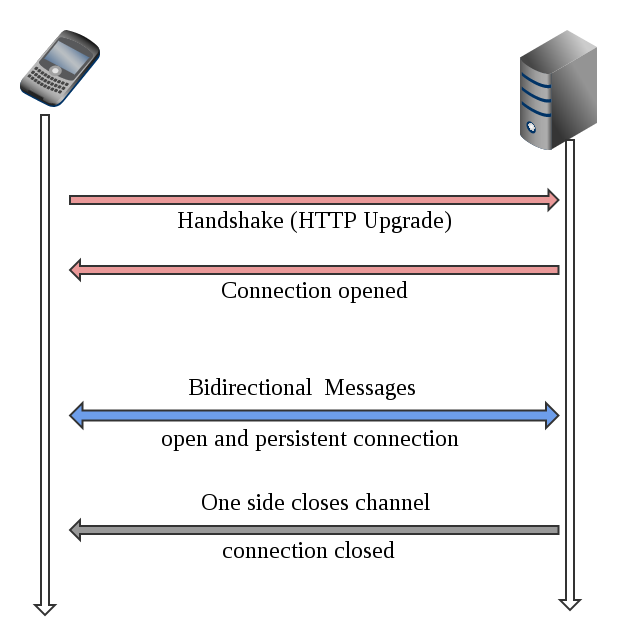
\includegraphics[scale=0.3]{websocket.png}
  \caption{Websocket handshake and communication}
\end{figure}

Another benefit to transport data over HTTP is that many existing HTTP security mechanisms also apply to websocket.
With this unified security model, a list of standard HTTP security methods could be applied to a websocket connection.
For example, the same encryption as HTTPS using TLS/SSL. It's the same way to configure TLS encryption for websocket as you do for HTTPS with
certificates. In HTTPS, the client and server first establish a secure envelop which begin with HTTP protocol. Websocket Secure (WSS) use
the exactly the same way with handshake in HTTP, then upgrade to websocket protocol. 

\begin{figure}[tbph]
  \centering
  \label{fig:wss}
  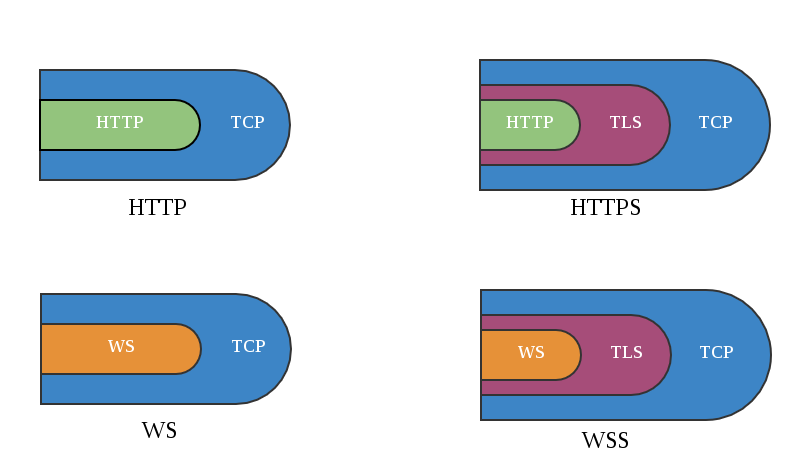
\includegraphics[scale=0.3]{wss.png}
  \caption{HTTPS and Websocket Secure}
\end{figure}

\subsection{HTTP Gateway} \label{HTTP Gateway}

One of the key concept of GNU Artanis is the HTTP Gateway. As mentioned earlier in this paper, HTTP Gateway is not a new concept,
for it's transparent in many server program.

The HTTP Gateway, as described intuitively, is a portal between client and customized protocol processing module of the server program,
and taking the HTTP negotiation to allow them to share information by communicating with the protocol over HTTP.

\begin{figure}[tbph]
  \centering
  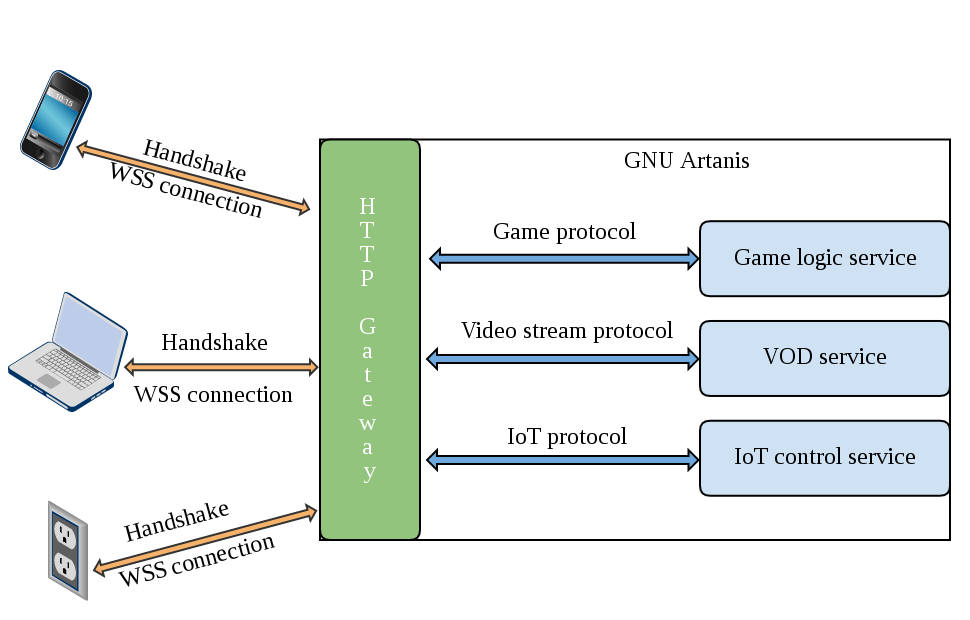
\includegraphics[scale=0.25]{httpgw.png}
  \caption{HTTP Gateway architecture in GNU Artanis}
  \label{fig:httpgw}
\end{figure}

The Figure \ref{fig:httpgw} shows the HTTP Gateway architecture in GNU Artanis.
Obviously, it takes advantage of the convenience in the server core of GNU Artanis to provide arbitrary protocol services in the
natural of websocket. Beyond the web server, it becomes a {\it generic server}, which handles connections in various protocols in the
same time.

What's the value of a {\it generic server}?

A {\it generic server} seems useless and meaningless in the past. Because most of the application of server programs are for dedicated
protocol, and to provide single service as its main duty.

For the {\it dedicated server}, FTP, HTTP as in web service, game server, IRC, etc. Usually, the remote server starts a service program
as a daemon listening on a TCP/UDP port according to a convention, and provides just one service in a dedicated protocol. Such a decoupled
pattern is obviously meets the KISS (Keep It Stupid and Simple) principle. Moreover, when one service is down, it won't effect the others.

For the {\it generic server}, people don't have to listen on many TCP ports, there's just one port, 80 or 443 (for HTTPS). And the HTTP
Gateway will dispatch the requests to the related service, and maintain the long live session for each connection in a high concurrent way.
In the simplest way, all the services are running in GNU Artanis rather than standalone, and it's good for quick developing then deployment.
But it's tight coupled, if one of the services is broken, the whole GNU Artanis may down. Fortunately, it is allowed to make each service
standalone, similar to CGI, but in bytevector way according to websocket configuration, rather than HTTP requests redirecting.

\subsection{Concurrency}

The eternal subject of server side development is always concurrency.
Many years ago, the industry has been focusing on {\it C10K} problem dealing with at least $10,000$ connection concurrently.
Nowadays, it's becoming {\it C10M} which means at least 10 million connections concurrently.

No matter how the number is increasing, the main purpose is to hold more connections concurrently as possible.
Unfortunately, it is useless if one just purchase stronger machines with more rams. In this way, the performance of single connection
processing could be higher, but increase few connections concurrently.

The bottleneck is not the performance of machine, but the algorithm of events dispatching. The traditional select() and poll() are outdated,
for their $O(n)$ complexity drags the performance when it tries to query large number of the ready file descriptors. The modern epoll() has
constant time complexity for that, say $O(1)$, and obviously win the title.

\subsubsection{Non-blocking with Epoll} \label{Non-blocking with Epoll}

\section{Some features in GNU Artanis} \label{Some features in GNU Artanis}

In spite of the server core, there're some notable features in GNU Artanis.

\subsection{RESTful}

REST stands for representational state transfer (REST), which is an architectural style consisting of a coordinated set of components, connectors,
and data elements within a distributed hypermedia system, where the focus is on component roles and a specific set of interactions between data
elements rather than implementation details.

Its purpose is to induce performance, scalability, simplicity, modifiability, visibility, portability, and reliability.
REST is the software architectural style of the World Wide Web.

To the extent that systems conform to the constraints of REST they can be called RESTful. RESTful systems typically, but not always,
communicate over Hypertext Transfer Protocol (HTTP) with the same HTTP verbs (GET, POST, PUT, DELETE, etc.) that web browsers use to retrieve web
pages and to send data to remote servers. REST systems interface with external systems as web resources identified by Uniform Resource Identifiers
(URIs).

The name "Representational State" is intended to evoke an image of how a well-designed Web application behaves: a network of web pages
(a virtual state-machine), where the user progresses through the application by selecting links (state transitions), resulting in the next page
(representing the next state of the application) being transferred to the user and rendered for their use.

\lstinputlisting{restful.scm}

\subsection{MVC}

Model$-$View$-$Controller (MVC) is a software architectural pattern for implementing user interfaces on computers. It divides a given software
application into three interconnected parts, so as to separate internal representations of information from the ways that information is
presented to or accepted from the user. Traditionally used for desktop graphical user interfaces (GUIs), this architecture has become extremely
popular for designing web applications.

The {\it Model} is the unchanging essence of the application/domain. And there'll be more than one interfaces with the {\it Model}, they're called
{\it Views}. The {\it Views} could be GUI, CLI or API. Although {\it Views} are very often graphical, they don’t have to be.
A {\it Controller} is an object that lets you manipulate a {\it View}. In a brief, {\it Controller} handles the input whilst the view handles the
output \citep{deacon2009model}.

GNU Artanis provides CLI tools for generating MVC template code, this will be introduced in \ref{CLI tools}.

\subsection{Relational Mapping}

Usually, Relational Mapping stands for ORM (Object Relational Mapping).
It is a programming technique for converting data between incompatible type systems in object-oriented programming languages.
This creates, in effect, a "virtual object database" that can be used from within the programming language.

In object-oriented programming, data-management tasks act on object-oriented (OO) objects that are almost always non-scalar values.
For example, consider an address book entry that represents a single person along with zero or more phone numbers and zero or more addresses.
This could be modeled in an object-oriented implementation by a "Person object" with attributes/fields to hold each data item that the entry
comprises: the person's name, a list of phone numbers, and a list of addresses. The list of phone numbers would itself contain "PhoneNumber objects"
and so on. The address-book entry is treated as a single object by the programming language (it can be referenced by a single variable containing a
pointer to the object, for instance). Various methods can be associated with the object, such as a method to return the preferred phone number,
the home address, and so on.

However, many popular database products such as SQL database management systems (DBMS) can only store and manipulate scalar values such as integers
and strings organized within tables. The programmer must either convert the object values into groups of simpler values for storage in the database
(and convert them back upon retrieval), or only use simple scalar values within the program. Object-relational mapping implements the first approach.
The heart of the problem involves translating the logical representation of the objects into an atomized form that is capable of being stored in the
database, while preserving the properties of the objects and their relationships so that they can be reloaded as objects when needed.
If this storage and retrieval functionality is implemented, the objects are said to be persistent.


\subsection{Web caching}

A web cache (or HTTP cache) is an information technology for the temporary storage (caching) of web documents, such as HTML pages and images,
to reduce bandwidth usage, server load, and perceived lag. A web cache system stores copies of documents passing through it; subsequent requests
may be satisfied from the cache if certain conditions are met. A web cache system can refer either to an appliance, or to a computer program.

\subsection{Sessions}

HTTP sessions allows associating information with individual visitors.

A session is a semi-permanent interactive information interchange, also known as a dialogue, a conversation or a meeting, between two or more
communicating devices, or between a computer and user. A session is set up or established at a certain point in time, and then
torn down at some later point. An established communication session may involve more than one message in each direction. A session is typically,
but not always, stateful, meaning that at least one of the communicating parts needs to save information about the session history in order to be
able to communicate, as opposed to stateless communication, where the communication consists of independent requests with responses.

Traditionally, there're three kinds of session management in GNU Artanis:

\begin{itemize}
\item {\it Simple}, use hashtables for storing sessions in the memory;
\item {\it Filesystem}, use files for storing sessions;
\item {\it Database}, use Database for storing sessions.
\end{itemize}

\subsection{CLI tools} \label{CLI tools}

Providing CLI tools is becoming a fashion for most of the frameworks.
Basically, there're four commands in GNU Artanis:

To initialize a new application folder:
\begin{lstlisting}
  art create project-name
\end{lstlisting}

And the {\it draw} command is useful to generate MVC template code to save developers work:
\begin{lstlisting}
  art draw [controller/model] name
\end{lstlisting}
Note that {\it Views} are generated along with {\it Controllers}.

Sometimes it's necessary to move from one database vendor to another, or to upgrade the version of database software being used.
So the database migration could be useful to reconstruct the schema and tables, then import all the data to the new environment automatically.
\begin{lstlisting}
  art migrate operator name
\end{lstlisting}

The last but not least, the {\it work} command is used to start the server, and establish the service listening on the specified port.
\begin{lstlisting}
  art work
\end{lstlisting}

\subsection{Security}

\section{Conclusion}


\appendix
\section{Appendix Title}

This is the text of the appendix, if you need one.

\acks

Acknowledgments, if needed.

% We recommend abbrvnat bibliography style.

\bibliographystyle{unsrtabbrvnat}

% The bibliography should be embedded for final submission.
\softraggedright

\bibliography{mmrref}

\end{document}
